\chapter{Implementation Details}
\label{chap:implementation}

This chapter delves into the specific implementation details of the C2 server, the Go-based implants, and the React web client. Key code structures, algorithms, and challenging aspects are discussed.

\begin{figure}[H]
    \centering
    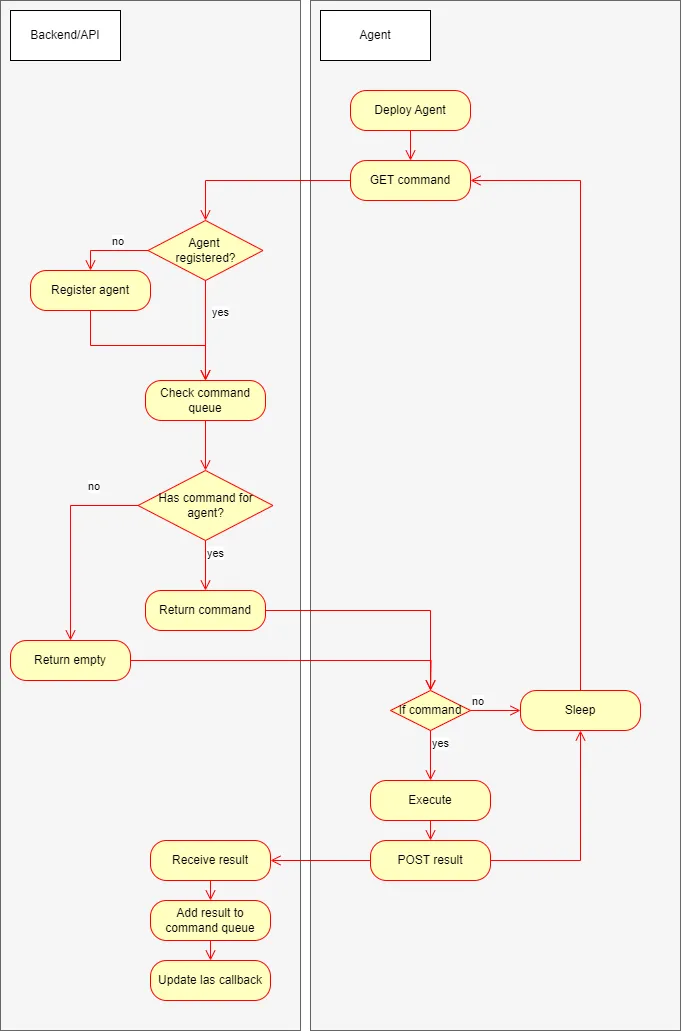
\includegraphics[width=0.8\textwidth]{../includegraphics/diagramm.png} % Ensure path is correct
    \caption{Architectural diagram illustrating the interaction between the Go-based implant, the C2 server, and the React web interface. It shows the agent deployment and communication flow.}
    \label{fig:architecture_diagram}
\end{figure}

\section{C2 Server Implementation (Go \& Gin Gonic)}
\subsection{Project Structure}
The Go-based C2 server, `awesomeProject`, is structured to promote modularity and maintainability. The typical directory layout includes:
\begin{itemize}
    \item \texttt{main.go}: The entry point of the application. It initializes the Gin Gonic router, sets up database connections (utilizing a GORM instance, e.g., `config.DB`), configures routes by calling `routes.SetupRouter()`, and starts the HTTP server. It may also initialize periodic tasks, such as updating inactive implant statuses.
    \item \texttt{config/}: Contains application-wide configurations, most notably the database connection setup (e.g., GORM initialization for \texttt{config.DB}) and potentially JWT secret keys (although the provided code has `jwtSecret` in `controllers/auth.go`).
    \item \texttt{routes/}: Defines all API endpoints. A central \texttt{routes.go} typically contains a `SetupRouter` function that initializes the Gin engine and groups public, implant-facing, and operator-facing (protected) routes, associating them with their respective controller handlers.
    \item \texttt{controllers/}: Houses the Gin handler functions that process incoming HTTP requests, interact with services or database layers, and formulate HTTP responses. Key controller files include:
        \begin{itemize}
            \item \texttt{auth.go}: Manages user authentication, with functions like `Register` and `Login`.
            \item \texttt{implant\_controllers.go}: Contains the core logic for implant interactions, such as `CheckinImplant`, `ImplantClientFetchCommands` (for implants to get tasks), `HandleCommandResult`, `GenerateImplant` (creates a DB record), `DownloadConfiguredImplant` (patches and serves binary), `GetUserImplants` (for dashboard), `SendCommand` (from dashboard to implant), `DashboardGetCommandsForImplant` (for dashboard history), `DeleteImplant`, `HandleLivestreamFrame`, and `GetScreenshotsForImplant`.
            \item \texttt{command\_controller.go}: While much command logic is within \texttt{implant\_controllers.go}, this could be used for more specialized command operations or historical data aggregation if expanded.
        \end{itemize}
    \item \texttt{middleware/}: Contains custom Gin middleware. A crucial piece is \texttt{auth.go} (or similar name), which provides `AuthMiddleware()` for JWT-based authentication, protecting operator-specific API endpoints.
    \item \texttt{models/}: Defines GORM data structures (structs) that map to database tables. These include:
        \begin{itemize}
            \item \texttt{user.go}: The `User` model with username and hashed password.
            \item \texttt{implant.go}: The `Implant` model storing metadata like unique token, status, OS, last seen IP, etc.
            \item \texttt{command.go}: The `Command` model for tasks assigned to implants, including their status and output.
            \item \texttt{screenshot\_info.go}: The `ScreenshotInfo` model for metadata of captured screenshots.
            \item \texttt{fs\_entry.go}: `FileSystemEntry` and `FileSystemListing` structs for file system browsing results.
        \end{itemize}
    \item \texttt{database/}: Provides a data access layer, containing functions that perform CRUD operations and other database queries using the GORM `config.DB` instance. This abstracts complex queries from the controllers (e.g., `GetImplantsByUserID`, `GetPendingCommandsForImplant`, `MarkCommandAsExecuted`, `CreateImplant`).
    \item \texttt{binaries/}: This directory stores pre-compiled base implant executables (e.g., \texttt{base\_client\_windows.exe}, \texttt{base\_client\_linux}). These are used as templates for the `DownloadConfiguredImplant` functionality, where they are patched with specific configurations.
\end{itemize}
This organization separates concerns, making the C2 server's codebase easier to navigate, test, and extend. Implant management, command queuing and execution, and user authentication are handled by dedicated modules interacting primarily through the database.

\subsection{API Endpoint Handling}
The C2 server exposes several RESTful API endpoints for communication with both the implants and the operator's web client. The Gin Gonic framework is utilized for routing and request handling. Below are examples of key endpoint definitions and their corresponding controller logic:

\begin{minted}{go}
// routes/routes.go
// SetupRouter initializes and configures the Gin engine with all application routes.
func SetupRouter() *gin.Engine {
    r := gin.Default() // Creates a Gin router with default middleware (logger, recovery).

    // Public routes for implant communication
    r.POST("/checkin", controllers.CheckinImplant)
    r.GET("/implant-client/:unique_token/commands", controllers.ImplantClientFetchCommands)
    r.POST("/command-result", controllers.HandleCommandResult)
    r.POST("/livestream-frame", controllers.HandleLivestreamFrame)

    // Public routes for user authentication
    r.POST("/register", controllers.Register)
    r.POST("/login", controllers.Login)

    // Protected routes for the Dashboard UI, requiring authentication
    protected := r.Group("/api")
    protected.Use(middleware.AuthMiddleware()) // Applies authentication middleware
    {
        // Implant management and interaction
        protected.GET("/implants", controllers.GetUserImplants)
        protected.POST("/generate-implant", controllers.GenerateImplant) // Creates implant record
        protected.POST("/send-command", controllers.SendCommand)
        protected.GET("/implants/:implant_id/commands", controllers.DashboardGetCommandsForImplant)
        protected.DELETE("/implants/:implant_id", controllers.DeleteImplant)
        // Patches and serves the implant binary
        protected.POST("/implants/:implant_id/download-configured", controllers.DownloadConfiguredImplant)
        protected.GET("/implants/:implant_id/screenshots", controllers.GetScreenshotsForImplant)
    }
    return r
}

// Example: controllers/implant_controller.go (Conceptual snippet for CheckinImplant)
// CheckinImplant handles implant registration and periodic check-ins.
func CheckinImplant(c *gin.Context) {
    var payload struct { // Simplified payload for example
        ImplantID string `json:"implant_id"` // This is unique_token from implant
        PWD       string `json:"pwd"`
    }
    if err := c.ShouldBindJSON(&payload); err != nil {
        c.JSON(http.StatusBadRequest, gin.H{"error": "Invalid payload: " + err.Error()})
        return
    }

    // Logic to update implant status in the database (e.g., using GORM via config.DB):
    // - Find implant by payload.ImplantID (which is its unique_token)
    // - Update 'last_seen' timestamp to time.Now()
    // - Update 'status' to "online"
    // - Update 'ip_address' with c.ClientIP()
    // - Update 'deployed' to true
    
    c.JSON(http.StatusOK, gin.H{"status": "checked_in", "message": "Implant check-in successful"})
}
\end{minted}
Other important controllers include `SendCommand`, which queues a new command for an implant by creating a database record with "pending" status. `HandleCommandResult` updates the command record with the output and "executed" status; it includes special logic for saving screenshot data to files if the output indicates a screenshot. `ImplantClientFetchCommands` allows an implant to retrieve its pending commands. `DownloadConfiguredImplant` is critical for implant delivery, as detailed next.

\subsection{Implant Generation and Configuration}
The C2 server facilitates the generation of customized implant binaries by patching pre-compiled base executables. This process avoids the need for a Go compiler on the C2 server for each implant request. The implant's Go source code itself uses the \texttt{go:embed} directive to include placeholder files which are read at runtime.

The implant source code (which is compiled into the base binaries stored on the C2) contains placeholders like:
\begin{itemize}
    \item \texttt{c2\_address.txt} (embedded content): Contains a placeholder string like \verb|C2_IP_PLACEHOLDER_STRING_PADDING_TO_64_BYTES_XXXXXXXXXXXXXXXXXXXXX|
    \item \texttt{placeholder.txt} (embedded content, for implant ID): Contains a placeholder UUID like \verb|deadbeef-0000-0000-0000-000000000000|
\end{itemize}

When an operator requests a new implant through the web UI:
\begin{enumerate}
    \item The C2 server (via the `GenerateImplant` controller) creates a new implant record in the database, generating a cryptographically secure unique ID (e.g., UUID) for it. The target OS (Windows/Linux) is also stored.
    \item When the operator chooses to download this configured implant (via the `DownloadConfiguredImplant` controller), they provide the C2 server's accessible IP address or domain name (and port) in the request.
    \item The C2 server reads the appropriate pre-compiled base implant binary (e.g., \texttt{binaries/base\_client\_windows.exe} or \texttt{binaries/base\_client\_linux}) from its file system into a byte slice.
    \item The C2 server then performs in-memory binary patching on this byte slice:
        \begin{itemize}
            \item It uses `bytes.LastIndex` to find the byte sequence corresponding to the implant ID placeholder (e.g., \texttt{tokenPlaceholder} variable in the controller). This sequence in the binary is then overwritten with the newly generated unique ID for this implant.
            \item Similarly, it uses `bytes.LastIndex` to find the C2 address placeholder (e.g., \texttt{c2Placeholder} variable). This sequence is overwritten with the C2 server address provided by the operator. The placeholders are padded to a fixed length to ensure the patching is a simple overwrite.
        \end{itemize}
    \item The modified (patched) binary byte slice is then streamed to the operator for download with an appropriate filename (e.g., \texttt{implant\_[unique\_token]\_windows.exe}).
\end{enumerate}
This on-demand patching of pre-compiled executables ensures each implant is uniquely identifiable and configured to communicate with the correct C2 server instance, without requiring on-the-fly compilation on the server. The implant, when run, reads these patched values from its embedded resources.

\subsection{Managing Implant State and Commands}
The C2 server relies on a relational database (interacted with via GORM, using the `config.DB` instance) to persist and manage all implant-related data, including their state, pending commands, and command history.

\begin{description}
    \item[Implant State] Information about each implant is stored in a dedicated table, mapped to the `models.Implant` GORM struct. This includes:
        \begin{itemize}
            \item \texttt{unique\_token}: A unique identifier for the implant, used in API paths and for linking commands.
            \item \texttt{user\_id}: Associates the implant with the operator who generated it.
            \item \texttt{status}: The current operational status (e.g., "new", "online", "offline"). This is updated upon check-ins (`CheckinImplant`), when an implant fetches commands (`ImplantClientFetchCommands`), submits results (`HandleCommandResult`), sends livestream frames (`HandleLivestreamFrame`), or by a periodic server-side task that marks long-unseen implants as "offline" (e.g., `database.UpdateStatusForInactiveImplants`).
            \item \texttt{target\_os}: The operating system of the implant ("windows", "linux").
            \item \texttt{last\_seen}: A timestamp indicating the last time the implant communicated with the C2.
            \item \texttt{ip\_address}: The last known IP address of the implant, updated during check-ins.
            \item \texttt{deployed}: A boolean flag, typically set to `true` after the first successful check-in.
        \end{itemize}

    \item[Commands and Results] Commands intended for implants, along with their execution status and results, are stored in a table mapped to the `models.Command` GORM struct. This includes:
        \begin{itemize}
            \item \texttt{implant\_id}: The \texttt{unique\_token} of the target implant.
            \item \texttt{command}: The actual command string to be executed by the implant.
            \item \texttt{status}: The lifecycle state of the command (e.g., "pending", "executed"). When an operator issues a command via the `SendCommand` controller, a new record is inserted with "pending" status.
            \item \texttt{output}: Stores the textual output or result received from the implant after execution. For screenshots, this field stores a message indicating where the image file was saved on the C2 server (e.g., "Screenshot saved to C2 server at: \texttt{c2\_screenshots/...}").
            \item \texttt{created\_at} and \texttt{updated\_at}: Timestamps for tracking command issuance and completion.
        \end{itemize}
        Implants poll the \texttt{/implant-client/:unique\_token/commands} endpoint (`ImplantClientFetchCommands` controller), which queries the database for "pending" commands for that specific implant using `database.GetPendingCommandsForImplant`. After execution, the implant sends results to \texttt{/command-result} (`HandleCommandResult` controller), which then updates the command's status to "executed" and records the output using `database.MarkCommandAsExecuted`.

    \item[Livestream Data] Livestream frames sent to \texttt{/livestream-frame} (`HandleLivestreamFrame` controller) are saved directly to the C2 server's filesystem under a directory specific to the implant (e.g., \texttt{c2\_screenshots/[implant\_token]/livestream\_frame\_[timestamp].png}).

    \item[Concurrency] The Gin web framework inherently handles concurrent HTTP requests from multiple operators and implants by processing each request in a separate goroutine. GORM, when used with a suitable database system (like PostgreSQL or MySQL), manages concurrent database access. The database connection pool configured with GORM helps in efficiently handling multiple simultaneous database operations. JWTs provide stateless authentication, further simplifying concurrent session management.
\end{description}

\section{Implant Implementation (Go)}
The implants are standalone Go executables designed for cross-platform compatibility and incorporating various functionalities for remote control and data gathering.

\subsection{Core Loop and Communication}
The implant's main operational logic resides in its \texttt{main.go} file. After initial setup, which includes daemonization and self-deletion scheduling, the implant enters a continuous loop.
(Refers to your `implant/main.go` structure)
\begin{minted}{go}
// implant/main.go (simplified conceptual structure)

//go:embed placeholder.txt
var implantIDBytes []byte // Embedded implant ID placeholder

//go:embed c2_address.txt
var c2AddressBytes []byte // Embedded C2 address placeholder

const checkInInterval = 5 * time.Second

var (
    exePath string // Path to the currently running implant executable
    gOriginalLauncherPath string // Path to the initial launcher, passed via env
    // ... other global vars like C2 URLs
)

func main() {
    var err error
    exePath, err = os.Executable() // Path of the CURRENTLY executing file
    if err != nil {
        // Handle error, perhaps log and exit
        os.Exit(1)
    }

    isBackgroundProcess := (os.Getenv(backgroundMarkerEnvVar) == "1")

    if !isBackgroundProcess {
        // This is the initial execution. Relaunch self in background.
        // Call platform-specific relaunchAsDaemonInternal, passing exePath as the
        // original launcher path to be stored in gOriginalLauncherPath by the child.
        // relaunchAsDaemonInternal will copy exePath and run the copy.
        // The original launcher (this process) exits after successful relaunch.
        // ... relaunch logic ...
        os.Exit(0)
    }

    // --- We ARE the background process ---
    os.Unsetenv(backgroundMarkerEnvVar) // Clear marker
    gOriginalLauncherPath = os.Getenv(originalPathEnvVar) // Get original launcher path
    os.Unsetenv(originalPathEnvVar) // Clear for security

    if !initializeConfig() { // Parses embedded C2_ADDRESS & IMPLANT_ID
        os.Exit(1) // Exit if config is invalid
    }

    // Schedule self-deletion in a separate goroutine.
    // This targets both the current running implant (exePath) and the
    // original launcher (gOriginalLauncherPath).
    if doSelfDelete != nil {
        go func() {
            time.Sleep(2 * time.Second) // Brief delay for implant startup
            doSelfDelete(exePath, gOriginalLauncherPath)
        }()
    }

    // Main operational loop
    for {
        checkIn() // Send heartbeat and PWD to C2
        // Pass current exePath (of this backgrounded process) AND the original launcher's path
        fetchAndExecuteCommands(exePath, gOriginalLauncherPath)
        time.Sleep(checkInInterval)
    }
}

// initializeConfig populates C2 URLs from embedded c2AddressBytes
// and verifies implantIDBytes.
func initializeConfig() bool { /* ... */ return true }

// checkIn sends a POST request to the C2 server's /checkin endpoint.
func checkIn() { /* ... */ }

// fetchAndExecuteCommands retrieves commands from the C2 server and processes them.
func fetchAndExecuteCommands(currentImplantExePath string, originalLauncherPath string) {
    // ... HTTP GET to C2's command URL for this implant ...
    // ... JSON unmarshal commands from response ...

    // For each command received:
    // Example command parsing:
    // if strings.HasPrefix(trimmedCmdStr, "fs_browse ") { listDirectory(...) }
    // else if trimmedCmdStr == "screenshot" { takeScreenshotAndSend() }
    // else if trimmedCmdStr == "livestream_start" { startLivestreamGoroutine() }
    // else if trimmedCmdStr == "self_destruct" {
    //     sendOutput(cmdToExec.ID, "Self-destruct initiated...")
    //     if doSelfDelete != nil {
    //         // Initiate deletion of current implant and original launcher
    //         doSelfDelete(currentImplantExePath, originalLauncherPath)
    //     }
    //     os.Exit(0) // Terminate implant to allow file deletion
    // }
    // else { /* Execute general shell command using os/exec */ }
    // ... After execution, call sendOutput() with results ...
}

// sendOutput sends the result of a command back to the C2 server.
func sendOutput(cmdID int, output string) { /* ... */ }

// doSelfDelete is a platform-specific function pointer.
var doSelfDelete func(selfExePath string, originalLauncherPath string)

// (Other platform-specific function pointers like takeScreenshot, setOSSpecificAttrs)
\end{minted}

\subsection{Daemonization Techniques}
To operate stealthily, implants employ platform-specific techniques to run as background processes without direct user interaction or visible console windows. The initial executable (launcher) is responsible for creating a detached, hidden copy of itself.

\subsubsection{Windows (\texttt{relaunch\_windows.go})}
The \texttt{relaunchDaemonWindows} function in \texttt{relaunch\_windows.go} handles daemonization on Windows systems:
\begin{itemize}
    \item The currently running executable's path (\texttt{currentExePath}, which is the initial launcher) is identified.
    \item This executable is copied to a new, often innocuously named file (e.g., \texttt{audiosrvhost\_[timestamp]\_[random].exe}) within the user's temporary directory (\texttt{os.TempDir()}).
    \item An \texttt{exec.Command} is prepared to run this newly copied executable.
    \item Crucially, two environment variables are set for the new process:
        \begin{itemize}
            \item \texttt{IMPLANT\_IS\_BACKGROUND\_XYZ123=1}: A marker indicating this new process is the daemonized instance.
            \item \texttt{IMPLANT\_ORIG\_LAUNCHER\_PATH\_XYZ789=[path\_to\_currentExePath]}: Stores the path of the original launcher, which the daemonized implant will need for self-deletion purposes.
        \end{itemize}
    \item The \texttt{SysProcAttr} of the command is configured with:
        \begin{itemize}
            \item \texttt{HideWindow: true}
            \item \texttt{CreationFlags: 0x08000000 \textbar \ 0x00000008} (CREATE\_NO\_WINDOW \textbar \ DETACHED\_PROCESS). These flags ensure the new process runs without a console window and is detached from the parent's console session.
        \end{itemize}
    \item The new process is started using \texttt{cmd.Start()}.
    \item The parent process (the initial launcher) then calls \texttt{cmd.Process.Release()} to detach from the child process, allowing the child to continue running independently.
    \item Finally, the initial launcher process (\texttt{currentExePath}) exits (\texttt{os.Exit(0)}). The backgrounded copy, upon starting, checks for the \texttt{IMPLANT\_IS\_BACKGROUND\_XYZ123} environment variable, retrieves the original launcher's path from \texttt{IMPLANT\_ORIG\_LAUNCHER\_PATH\_XYZ789}, and proceeds with its C2 operations.
\end{itemize}

\subsubsection{Linux (\texttt{platform\_linux.go})}
On Linux, daemonization is achieved by the \texttt{linuxRelaunchAsDaemon} function in \texttt{platform\_linux.go}:
\begin{itemize}
    \item The path of the executable to be daemonized (\texttt{originalLauncherExecutablePath}, which is the initial launcher) is taken as input.
    \item This executable is copied to a temporary file with a randomized name (e.g., \texttt{/tmp/implant\_[randomhex]}) and made executable.
    \item An \texttt{exec.Command} is prepared to run this temporary executable. The first argument to the command (\texttt{argv[0]}) is set to a desired spoofed name (e.g., \texttt{[kthreadd]}) to masquerade the process in listings.
    \item Similar to Windows, environment variables \texttt{IMPLANT\_IS\_BACKGROUND\_XYZ123=1} and \texttt{IMPLANT\_ORIG\_LAUNCHER\_PATH\_XYZ789=[originalLauncherExecutablePath]} are set for the new process.
    \item The \texttt{SysProcAttr} of the command is configured with \texttt{Setsid: true}. This creates a new session and detaches the process from the controlling terminal, making it a daemon.
    \item The new process is started using \texttt{cmd.Start()}.
    \item Immediately after successful start, the temporary executable file (\texttt{/tmp/implant\_[randomhex]}) is deleted from the filesystem using \texttt{os.Remove()}. This results in the daemonized process running from an unlinked file, a common "fileless" execution characteristic for the copied instance.
    \item The initial launcher process (\texttt{originalLauncherExecutablePath}) then exits (\texttt{os.Exit(0)}). The daemonized implant proceeds as described for the Windows case.
\end{itemize}
Additionally, the Linux implant attempts to further obfuscate its presence by calling \texttt{prctl(PR\_SET\_NAME, ...)} via CGo (in \texttt{proc\_rename\_linux.go}) to change its kernel thread name, although this name is typically truncated to 15 characters.

\begin{figure}[H]
    \centering
    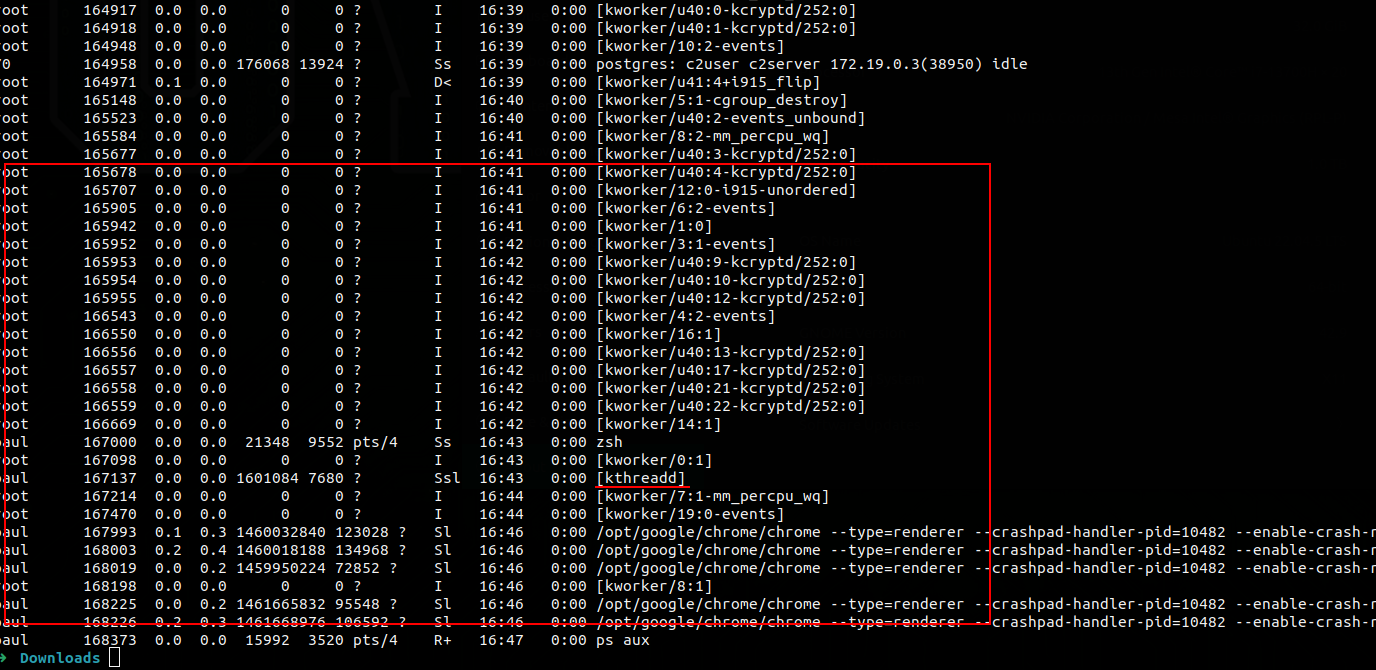
\includegraphics[width=0.8\textwidth]{../screenshots/linux_process_list.png} % Ensure path is correct
    \caption{A screenshot from a Linux system showing the implant process masquerading with a common kernel thread name, `[kthreadd]` (actual name may vary based on implant configuration).}
    \label{fig:linux_process_masquerade}
\end{figure}

\subsection{Self-Deletion Mechanisms}
To minimize forensic artifacts, implants are designed to delete both the initial launcher executable and their own currently running executable file (the daemonized copy) upon receiving a \texttt{self\_destruct} command or potentially as a final cleanup step.

\subsubsection{Windows (\texttt{exec\_attrs\_windows.go})}
The \texttt{doSelfDeleteWindows} function orchestrates self-deletion on Windows:
\begin{description}
    \item[Deleting the Original Launcher] If an \texttt{originalLauncherPath} is provided (and is different from the current implant's path), the \texttt{deleteFileViaBatch} function is called. This function:
        \begin{itemize}
            \item Creates a temporary batch script (e.g., \texttt{del\_file\_proc[PID]\_time[NANO].bat}) in \texttt{os.TempDir()}.
            \item The batch script contains commands to forcefully delete the specified \texttt{originalLauncherPath} and then delete the batch script itself.
            \item This batch script is executed as a new, detached, and hidden process (\texttt{cmd.exe /C [batch\_file\_path]} with \texttt{CREATE\_NO\_WINDOW | DETACHED\_PROCESS}). The parent Go process does not wait for its completion.
        \end{itemize}
    \item[Marking the Current Implant for Deletion] The \texttt{markFileForDeleteOnCloseAndPosixSemantics} function is called with the path to the currently running implant executable (\texttt{selfExePath}). This function:
        \begin{itemize}
            \item Opens a handle to \texttt{selfExePath} with \texttt{DELETE} access and \texttt{FILE\_SHARE\_DELETE}.
            \item Calls the Windows API \texttt{SetFileInformationByHandle} with the class \texttt{FileDispositionInformationEx} (value 64) and a structure containing the flags \texttt{FILE\_DISPOSITION\_FLAG\_DELETE | FILE\_DISPOSITION\_FLAG\_POSIX\_SEMANTICS}.
            \item This marks the file such that it will be deleted by the operating system once the last handle to it is closed (i.e., when the implant process exits). The POSIX semantics flag also helps prevent new handles from being opened to the file.
        \end{itemize}
\end{description}
After initiating these deletion mechanisms, if the implant receives a \texttt{self\_destruct} command, it will call \texttt{os.Exit(0)} to allow the file system operations to complete.

\subsubsection{Linux (\texttt{platform\_linux.go})}
On Linux, the \texttt{linuxScheduleSelfDeleteGrandchild} function handles deletion:
\begin{description}
    \item[Deleting the Original Launcher] If \texttt{originalLauncherPath} is valid and different from \texttt{selfExePath}, a shell command is constructed: \verb|sleep 1 && rm -f "[quoted_originalLauncherPath]"|.
        \begin{itemize}
            \item This command is executed using \texttt{exec.Command("sh", "-c", ...)}.
            \item \texttt{SysProcAttr} is set with \texttt{Setsid: true} to detach the deletion process.
            \item The command is started with \texttt{cmd.Start()}, and a separate goroutine calls \texttt{cmd.Wait()} to reap the child process and prevent it from becoming a zombie.
        \end{itemize}
    \item[Deleting the Current Implant Executable] A similar shell command is constructed for \texttt{selfExePath}: \verb|sleep 3 && rm -f "[quoted_selfExePath]"|. This also uses a detached process with \texttt{Setsid: true} and is reaped by a goroutine. The slightly longer sleep (3 seconds) is to give the implant a moment to fully exit if the self-destruct command also triggers \texttt{os.Exit(0)}.
\end{description}
Upon a \texttt{self\_destruct} command, the implant calls \texttt{os.Exit(0)}, allowing these scheduled \texttt{rm} commands to delete the unlinked (for the daemonized copy) and original launcher files.

\subsection{Screenshot and Livestreaming}
Implants can capture screenshots of the host's desktop and stream them to the C2 server.

\subsubsection{Screenshot Capabilities (\texttt{screenshot\_linux.go}, \texttt{exec\_attrs\_windows.go})}
The \texttt{takeScreenshot} function pointer is assigned a platform-specific implementation:
\begin{description}
    \item[Windows] Utilizes the \texttt{github.com/kbinani/screenshot} package. It captures the primary display's bounds using \texttt{screenshot.GetDisplayBounds(0)} and then captures the rectangle with \texttt{screenshot.CaptureRect()}. The resulting image is encoded to PNG format and then Base64 encoded for transmission.
    \item[Linux] The \texttt{linuxTakeScreenshot} function attempts a series of external screenshot utilities commonly found on Linux systems, in order of preference (e.g., \texttt{grim} for Wayland, \texttt{maim} for X11, \texttt{import} from ImageMagick, \texttt{scrot}).
        \begin{itemize}
            \item For each utility, it first checks if the command exists using \texttt{exec.LookPath()}.
            \item It then tries to execute the utility with arguments that pipe the PNG output directly to standard output. If successful, this output is captured.
            \item If piping to stdout fails or is not supported by the utility, it attempts to save the screenshot to a temporary PNG file. This file is then read.
            \item The captured image data (from stdout or the temp file) is Base64 encoded.
            \item If all attempts fail, an error is returned.
        \end{itemize}
\end{description}
The Base64 encoded screenshot data is prefixed with \texttt{"screenshot\_data:"} and sent to the C2 server.

\subsubsection{Livestreaming Logic (\texttt{implant/main.go})}
Desktop livestreaming is initiated by the \texttt{livestream\_start} command from the C2:
\begin{itemize}
    \item Sets a flag \texttt{isLivestreamActive} to true.
    \item Creates a \texttt{stopLivestreamChan} channel.
    \item Launches the \texttt{runLivestream} function in a new goroutine.
    \item \texttt{runLivestream} uses a \texttt{time.NewTicker} (typically set for 1-second intervals, i.e., 1 FPS).
    \item On each tick, it calls the platform-specific \texttt{takeScreenshot()} function.
    \item The Base64 encoded frame data is then sent to the C2 server's \texttt{/livestream-frame} endpoint via an HTTP POST request in a \texttt{LivestreamFramePayload}.
    \item The livestream continues until the \texttt{livestream\_stop} command is received, which closes the \texttt{stopLivestreamChan}, causing the \texttt{runLivestream} goroutine to terminate.
\end{itemize}

\subsection{File System Interaction (\texttt{fs\_utils.go})}
Implants provide capabilities to browse the remote file system and download files. These are primarily handled by functions in \texttt{fs\_utils.go}.
\begin{description}
    \item[\texttt{listDirectory(path string)}]
        \begin{itemize}
            \item Takes a directory path as input.
            \item Uses \texttt{os.ReadDir} to get a list of \texttt{os.DirEntry} items.
            \item For each entry, it calls \texttt{entry.Info()} to get \texttt{os.FileInfo}, from which it extracts the \texttt{Name}, \texttt{IsDir}, \texttt{Size}, \texttt{ModTime}, and \texttt{Mode().String()} (permissions).
            \item Constructs a \texttt{FileSystemListing} struct containing a slice of \texttt{FileSystemEntry} structs and sends this JSON-marshaled data to the C2.
        \end{itemize}
    \item[\texttt{listRoots()}]
        \begin{itemize}
            \item Provides a list of root directories.
            \item On Windows, it iterates from drive 'A' to 'Z', checking for existence with \texttt{os.Stat(drive + ":\\")}.
            \item On Linux and other Unix-like systems, it typically lists the root directory \texttt{"/"}.
            \item Returns a \texttt{FileSystemListing} similar to \texttt{listDirectory}.
        \end{itemize}
    \item[File Download (handled in \texttt{fetchAndExecuteCommands})]
        \begin{itemize}
            \item Triggered by an \texttt{fs\_download} command specifying a file path.
            \item Uses \texttt{os.ReadFile} to read the entire file content into a byte slice.
            \item The byte slice is then Base64 encoded.
            \item The encoded data is prefixed with \texttt{"file\_data\_b64:"} and sent to the C2 server as the command's output.
        \end{itemize}
\end{description}
The implant also supports the \texttt{cd} command, which uses \texttt{os.Chdir} to change the implant's current working directory. The updated PWD is reflected in subsequent check-ins.

\section{Web Client Implementation (React)}
The web client is a Single Page Application (SPA) built with React, providing the operator with an interface to interact with the C2 server and manage implants.

\subsection{Project Structure}
The React application's \texttt{src} directory is organized to separate concerns, typically including:
\begin{itemize}
    \item \texttt{App.js}: The root component of the application, responsible for setting up client-side routing (likely using `react-router-dom`, as evidenced by `useNavigate` and `Link` imports in components) and rendering top-level layout.
    \item \texttt{index.js}: The main entry point that renders the \texttt{App} component into the DOM.
    \item \texttt{components/}: This directory houses a collection of reusable UI components and potentially page-level views. Based on the provided code, key components include:
        \begin{itemize}
            \item \texttt{AuthForm.js}: Handles user registration and login forms.
            \item \texttt{Dashboard.js}: Serves as the main operational view after login. It displays the list of implants, provides controls for implant generation, download, deletion, and access to interactive features like the terminal, file explorer, and screenshot/livestream viewers. It also manages global UI elements like notifications and modals.
            \item \texttt{Terminal.js}: An interactive pseudo-terminal for sending commands to a selected implant and viewing output.
            \item \texttt{FileSystemExplorer.js}: A component for browsing the file system of a selected implant.
            \item \texttt{ScreenshotViewer.js}: A modal component for displaying individual screenshots in a gallery format or a live desktop stream.
            \item \texttt{DownloadOptionsModal.js}: A modal dialog for specifying the C2 server IP when downloading a configured implant.
            \item \texttt{GenerateImplantOSModal.js}: A modal for selecting the target OS when creating a new implant record.
            \item (Other modals like `DeleteConfirmationModal` are defined as sub-components or directly within `Dashboard.js`).
        \end{itemize}
    \item \texttt{services/} or \texttt{api/}: While not explicitly shown as a separate directory in the provided snippets, API calls to the C2 backend are made using the browser's `fetch` API directly within components (e.g., in `Dashboard.js`, `Terminal.js`, `AuthForm.js`). In larger applications, this logic might be abstracted into dedicated service modules.
    \item \texttt{hooks/}: Custom React hooks for encapsulating reusable stateful logic or side effects are a common pattern, although no specific custom hooks are detailed in the provided code.
    \item \texttt{context/} or \texttt{store/}: Global state management beyond component-level state and prop drilling is not explicitly demonstrated. The application appears to rely on:
        \begin{itemize}
            \item Local component state managed by `useState` and `useRef`.
            \item Passing state and callbacks down through props (prop drilling), for example, `displayNotification` and `openScreenshotViewer` functions from `Dashboard.js`.
            \item `localStorage` is utilized to persist the JWT authentication token and the operator's preferred default C2 IP address across sessions.
        \end{itemize}
        For more complex state interdependencies, React Context API or libraries like Redux/Zustand could be integrated.
    \item CSS files (\texttt{App.css}, \texttt{index.css}, \texttt{styles.css}): Standard CSS files for styling. The use of class names like `flex`, `bg-gray-900`, `rounded-lg` suggests the adoption of a utility-first CSS framework like Tailwind CSS.
\end{itemize}

\subsection{Key Components}
The React frontend is composed of several key components that enable operator interaction:
\begin{description}
    \item[\\texttt{Dashboard.js}] This is the central hub for operators. It fetches and displays a list of active and inactive implants from the C2 server\'s \\verb|/api/implants| endpoint, showing details like ID (Token), OS, Status, Last Seen, and IP Address. From here, operators can:
        \\begin{itemize}
            \\item Initiate the generation of new implant records via \\texttt{GenerateImplantOSModal.js}.
            \\item Configure and download implant binaries via \\texttt{DownloadOptionsModal.js}.
            \\item Delete implants (with confirmation).
            \\item Open an interactive \\texttt{Terminal.js} for a selected implant.
            \\item Launch \\texttt{ScreenshotViewer.js} to view collected screenshots or start a live desktop stream.
            \\item Open \\texttt{FileSystemExplorer.js} for a selected implant.
            \\item Manage a global C2 IP setting for implant downloads.
            \\item It also handles displaying system-wide notifications.
        \\end{itemize}

    \begin{figure}[H]
        \\centering
        \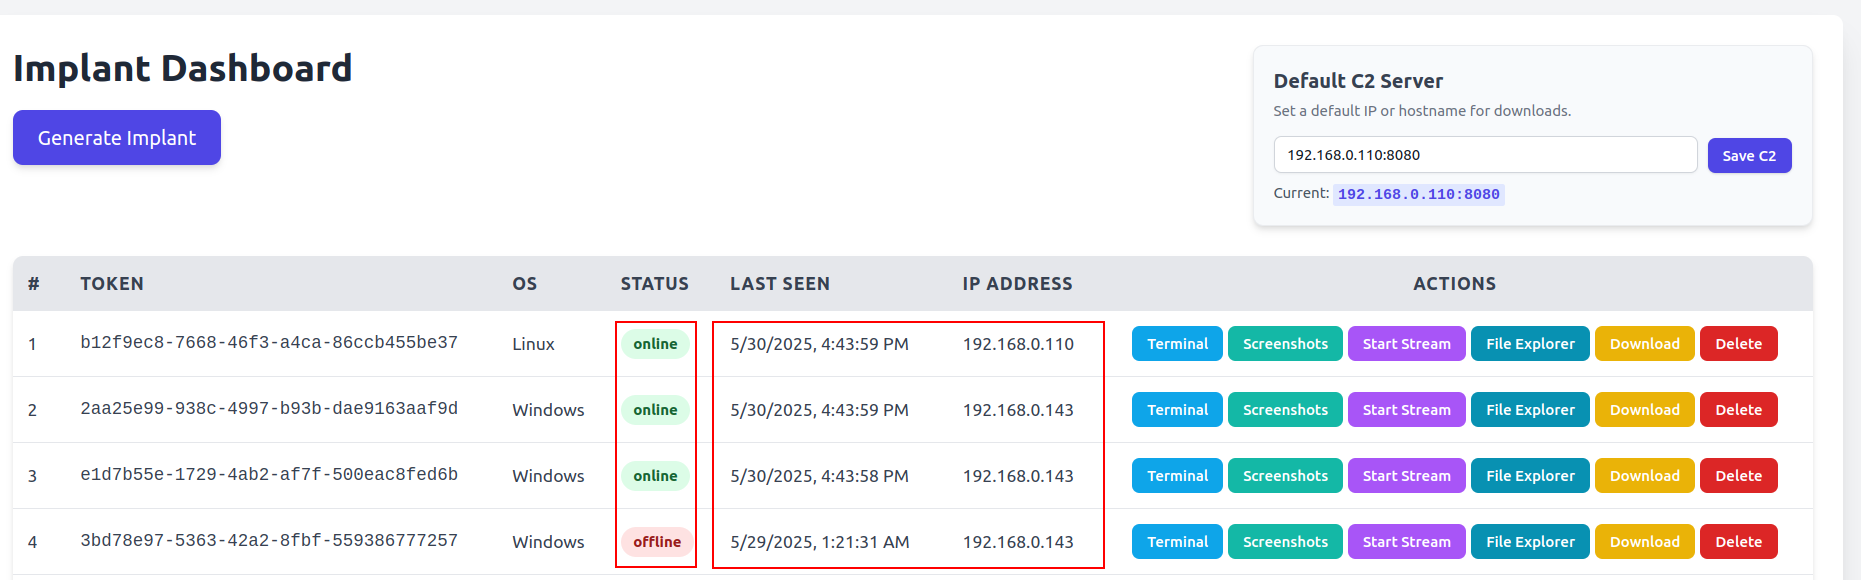
\includegraphics[width=0.8\\textwidth]{../screenshots/c2_dashboard.png} % Ensure path is correct
        \\caption{The C2 dashboard interface, showcasing the list of managed implants, their status, and available actions.}
        \\label{fig:c2_dashboard}
    \\end{figure}

    \\item[\\texttt{Terminal.js}] Provides an interactive pseudo-terminal interface for a specific implant.
        \\begin{itemize}
            \\item An input field allows the operator to type commands.
            \\item On submission, the command is sent to the C2 server via a POST request to \\verb|/api/send-command|, along with the selected implant\'s ID.
            \\item It periodically fetches new and updated command statuses/outputs for the active implant from the C2 server (e.g., \\verb|/api/implants/:implant_id/commands|) and displays the command history and output.
            \\item If a command output indicates a saved screenshot, it provides a button to open it in the \\texttt{ScreenshotViewer.js}.
        \\end{itemize}

    \begin{figure}[H]
        \\centering
        \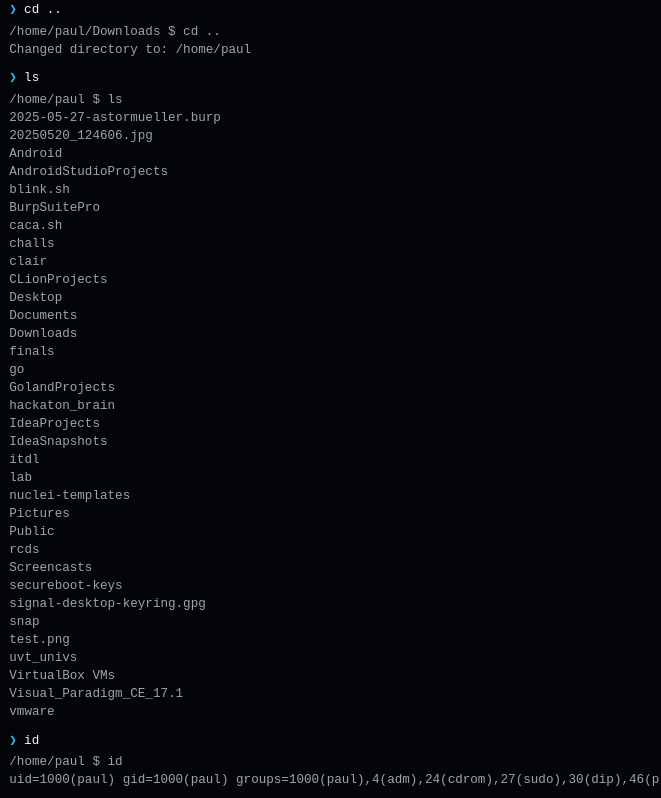
\includegraphics[width=0.8\\textwidth]{../screenshots/terminal.png} % Ensure path is correct
        \\caption{The interactive terminal within the C2 web interface, allowing operators to send commands to and receive output from an implant.}
        \\label{fig:c2_terminal}
    \\end{figure}

    \\item[\\texttt{FileSystemExplorer.js}] Renders a file and directory listing received from an implant (after an \\texttt{fs\\_browse} command). It allows:
        \\begin{itemize}
            \\item Navigation into subdirectories (by issuing new \texttt{fs\_browse} commands via `cd` equivalent logic or by clicking on directory entries which changes the `currentPath` state, triggering a new browse command).
            \\item Navigation up to parent directories.
            \\item Triggering file downloads by sending \texttt{fs\_download} commands for selected files.
            \\item It polls for command results similarly to the terminal.
        \\end{itemize}
    \\item[\\texttt{ScreenshotViewer.js}] A modal component responsible for displaying images.
        \\begin{itemize}
            \\item In 'gallery' mode, it displays individual screenshots fetched from the C2 server (e.g., from URLs like \\texttt{/c2\\_screenshots/:implant\\_id/:filename.png} which are served statically by the C2, paths obtained via \\verb|/api/implants/:implant_id/screenshots|). It provides navigation controls (next/previous, slideshow).
            \\item In 'livestream' mode, it continuously updates an \\texttt{<img>} tag with the latest frame fetched from the C2 (image paths are polled).

            \begin{figure}[H]
                \\centering
                \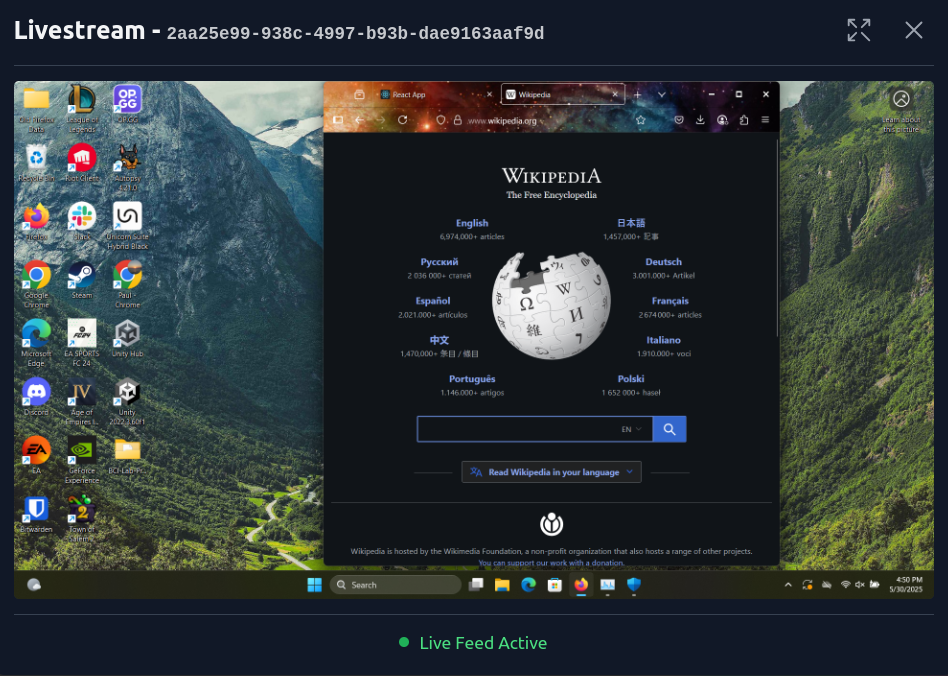
\includegraphics[width=0.8\\textwidth]{../screenshots/livestream.png} % Ensure path is correct
                \\caption{Example of the livestream feature, displaying a real-time screen capture from a compromised implant.}
                \\label{fig:livestream_example}
            \\end{figure}

            \\item Supports a fullscreen mode for better viewing.
            \\item When closed in 'livestream' mode, it can trigger a \\texttt{livestream\\_stop} command to be sent to the implant.
        \\end{itemize}
    \\item[Authentication Components (\\texttt{AuthForm.js})] Handles user registration and login.
        \\begin{itemize}
            \\item Makes POST requests to the C2 server's \verb|/register| and \verb|/login| endpoints.
            \\item Upon successful authentication, it stores the received JWT in `localStorage`.
            \\item Navigates the user to the \texttt{/dashboard}.
        \\end{itemize}
    \\item[Modal Components (\\texttt{GenerateImplantOSModal.js}, \texttt{DownloadOptionsModal.js})]
        \\begin{itemize}
            \\item \texttt{GenerateImplantOSModal.js}: A form allowing the operator to select the target OS (Windows/Linux) for a new implant. Triggers an API call to \verb|/api/generate-implant| to create the implant record in the C2 database.
            \\item \texttt{DownloadOptionsModal.js}: A form that appears when downloading a configured implant. It prompts the operator for the C2 server's IP address (pre-filled with a global default if set) which will be embedded into the implant binary. Triggers a POST request to \verb|/api/implants/:implant_id/download-configured|.
        \\end{itemize}
\end{description}

(Below is a conceptual React snippet for a simplified terminal input component)
\begin{minted}{js}
// Example: Simplified TerminalInput.js component (part of Terminal.js)
import React, { useState } from 'react';
// Assume 'apiService.sendCommandToImplant' is a function that POSTs to the C2.

function TerminalInput({ selectedImplantId, onCommandSent }) {
    const [command, setCommand] = useState('');
    const [isLoading, setIsLoading] = useState(false);


    const handleSubmit = async (event) => {
        event.preventDefault();
        if (!command.trim() || !selectedImplantId || isLoading) return;
        setIsLoading(true);

        try {
            // Example API call structure within Terminal.js:
            // const token = localStorage.getItem("token");
            // const res = await fetch("/api/send-command", {
            //   method: "POST",
            //   headers: { "Content-Type": "application/json", Authorization: `Bearer ${token}` },
            //   body: JSON.stringify({ implant_id: selectedImplantId, command: command }),
            // });
            // if (!res.ok) { /* handle error */ }
            // Optimistic UI update or rely on poller in Terminal.js
            console.log(`Sending command: ${command} to ${selectedImplantId}`);


            setCommand(''); // Clear input field
            if (onCommandSent) { // Callback might trigger immediate fetch or rely on existing poller
                onCommandSent();
            }
        } catch (error) {
            console.error("Error sending command:", error);
            // Handle error (e.g., display a notification to the user)
        } finally {
            setIsLoading(false);
        }
    };

    return (
        <form onSubmit={handleSubmit} className="flex items-center p-2">
            <span className="text-blue-400 mr-2">{">"}</span>
            <input
                type="text"
                value={command}
                onChange={(e) => setCommand(e.target.value)}
                placeholder="Enter command..."
                disabled={!selectedImplantId || isLoading}
                className="flex-grow bg-transparent focus:outline-none"
                autoFocus
            />
            <button type="submit" disabled={!selectedImplantId || !command.trim() || isLoading}
                    className="bg-blue-500 text-white px-3 py-1 rounded ml-2 hover:bg-blue-600 disabled:opacity-50">
                {isLoading ? "Sending..." : "Send"}
            </button>
        </form>
    );
}

export default TerminalInput;
\end{minted}

\subsection{State Management and API Interaction}
\begin{description}
    \item[State Management]
    The React application primarily employs component-level state management using React's built-in hooks:
    \begin{itemize}
        \item \texttt{useState}: Used extensively for managing local component data, such as input field values, lists of items (e.g., implants, commands, file entries), modal visibility, loading indicators, and error messages.
        \item \texttt{useEffect}: Manages side effects, including fetching initial data when a component mounts, setting up and tearing down intervals for polling.
        \item \texttt{useRef}: Utilized for accessing underlying DOM elements (e.g., `containerRef` in `Terminal.js` for scrolling, `viewerContentRef` in `ScreenshotViewer.js` for fullscreen) and for storing mutable values that do not trigger re-renders across the component lifecycle (e.g., `polling.current` flag, interval IDs).
    \end{itemize}
    For cross-component state or actions, the application relies on:
    \begin{description}
        \item[Prop Drilling] Callbacks and state values are passed down from parent components to children (e.g., `displayNotification` function and `openScreenshotViewer` function are passed from `Dashboard.js` to child components like `Terminal.js` and `FileSystemExplorer.js`).
        \item[\texttt{localStorage}] Used for persisting data across browser sessions, specifically the JWT authentication token (`token`) obtained after login and a user-configurable global C2 IP address (`dashboardGlobalC2IP`) used as a default for implant downloads.
    \end{description}
    While no global state management libraries like Redux or Zustand, or React's Context API, are explicitly shown in the provided snippets for application-wide state, these could be integrated if the complexity of state sharing grows.

    \item[API Interaction]
    Communication with the C2 server's RESTful API is handled using the browser's native \texttt{fetch} API:
    \begin{itemize}
        \item API calls are typically encapsulated within asynchronous functions (`async/await`) inside React components, often triggered by user interactions (e.g., button clicks) or by `useEffect` hooks (e.g., for initial data loading or polling).
        \item For requests to protected API endpoints (those under the `/api` group), the JWT stored in `localStorage` is retrieved and included in the `Authorization` header as a Bearer token (e.g., `headers: \{ 'Authorization': \`Bearer \$\{token\}\` \}`).
        \item Request bodies for `POST` or `PUT` methods are usually JSON, prepared using `JSON.stringify()`.
        \item Server responses are typically expected in JSON format and are parsed using `response.json()`.
        \item \textbf{Polling:} For real-time updates in the terminal, screenshot viewer (livestream), and file explorer, `setInterval` is used within `useEffect` hooks to periodically call relevant API endpoints. These intervals are cleared in the `useEffect` cleanup function to prevent memory leaks and unnecessary calls when the component unmounts or the polling condition changes. The `Dashboard.js` component also checks `document.hidden` to pause screenshot polling when the browser tab is not active.
    \end{itemize}

    \item[Error Handling and Loading States]
    \begin{description}
        \item[Error Handling] API calls made with `fetch` are wrapped in `try...catch` blocks to handle network errors or exceptions during the request/response cycle. Non-`2xx` HTTP status codes are checked (e.g., `if (!response.ok)`), and error messages are often parsed from the JSON response body. Errors are communicated to the user via a centralized notification system (the `Notification` component in `Dashboard.js`, triggered by the `displayNotification` function) or through component-specific error messages displayed in the UI.
        \item[Loading States] Boolean state variables (e.g., `loading` in `Terminal.js`, `isInitiallyLoading` and `isManuallyRefreshing` in `FileSystemExplorer.js`, `isLoadingInitial` in `ScreenshotViewer.js`) are used to track the asynchronous nature of API calls. These states control UI elements by:
            \begin{itemize}
                \item Disabling buttons or input fields during an operation to prevent duplicate submissions.
                \item Displaying loading indicators like spinners or textual messages (e.g., "Loading...", "Sending...").
                \item Conditionally rendering parts of the UI based on whether data is available or an operation is in progress.
            \end{itemize}
    \end{description}
\end{description}

\section{Challenges Encountered and Solutions}
Throughout the development of this C2 framework, several technical challenges were encountered:
\begin{itemize}
    \item Cross-Platform Nuances in Implants: Ensuring consistent behavior for daemonization, self-deletion, and screenshotting across Windows and Linux required careful use of Go's build tags (e.g., \\texttt{//go:build windows}) and platform-specific API calls or external utilities. For example, Windows file deletion required a combination of marking files for delete-on-close and using detached batch scripts for locked files, while Linux relied on detached \\texttt{rm} commands.
    \item Reliable Self-Deletion: Deleting an executable while it is running, or deleting its original launcher, is inherently tricky due to file locking by the OS. The solutions involved detached processes (batch scripts on Windows, \\texttt{sh -c} on Linux) and OS-specific APIs like \\texttt{SetFileInformationByHandle} on Windows.
    \item Process Hiding and Masquerading on Linux: While changing \\texttt{argv[0]} during the \\texttt{execve} syscall (achieved by setting \\texttt{cmd.Args[0]} in Go before \\texttt{cmd.Start()} for the daemonized copy) is effective for altering how the process appears in tools like \texttt{ps}, the \texttt{prctl(PR\\_SET\\_NAME)} call has limitations (e.g., 15-character limit, only affects thread name). A combination provides better, though not perfect, obfuscation.
    \item React State Management for Real-time Updates: Efficiently updating the UI for features like the livestreaming desktop view or the interactive terminal (which requires polling for new command outputs) without causing performance degradation or excessive re-renders required careful state management (primarily `useState`, `useEffect`), memoization where necessary (e.g., \\texttt{React.memo}, \\texttt{useMemo}, \\texttt{useCallback}, though not explicitly detailed in provided code, these are common optimizations), and ensuring polling intervals are managed correctly (cleared on unmount, paused when tab is hidden).
    \item Implant Configuration and Delivery: The method of patching pre-compiled base binaries with C2 addresses and implant IDs is efficient as it avoids needing a Go compiler on the C2 server. However, the placeholder strings and the patched information are stored as plain text within the binary. This means if an implant binary is captured, the C2 address can be easily extracted. More advanced C2s might use encrypted configuration blocks or staged loading to better protect this information. The current approach trades some operational security for simplicity in generation and deployment.
    \item Locating and Patching Embedded Placeholders in Pre-compiled Binaries: The implant generation relies on finding specific placeholder byte sequences within pre-compiled base binaries to patch in the unique implant ID and C2 server address. Ensuring these placeholders are unique enough not to appear elsewhere in the binary by chance, are of a fixed and known size, and that the patching process correctly overwrites them without corrupting the executable requires careful management of the base binary's compilation (ensuring placeholders exist) and the patching logic on the C2 server (using `bytes.LastIndex`). The implant then uses `go:embed` to access these (now patched) values from its embedded resources at runtime.
    \item Handling Concurrent Operations on the C2 Server: While Gin handles concurrent HTTP requests, ensuring that database operations are performed safely and without race conditions required reliance on GORM's capabilities and the underlying database's concurrency control mechanisms. For instance, updating implant 'last seen' times or command statuses from multiple concurrent implant check-ins needs to be handled correctly by the database.
    \item Robust Screenshot and Livestream File Management: Saving screenshot and livestream frames involves creating directories and files on the C2 server. Ensuring proper permissions, handling potential write errors, and organizing files in a structured way (e.g., \\texttt{c2\\_screenshots/[implant\\_token]/[filename]}) was necessary for reliable storage and retrieval by the frontend.
\end{itemize}

This chapter has provided an overview of the implementation details for the core components of the C2 framework. The choices made reflect a balance between functionality, cross-platform compatibility, and the foundational evasion techniques explored in this thesis.